\section{Results}
\label{sec:results}

\begin{table*}[t]
\caption{Cost of each strategy. Top: the \paramsM{}M-parameter model, all migration points and \seedsM{} seeds.
Middle: the \largeParams{}M-parameter model (\largeSeeds{} seeds, two migration points). Bottom: ResNet-18 on CIFAR-10
(\cifarSeeds{} seeds). Payload is the share of the full state's bytes. Peak is the largest excess held-out loss in
the \horizon{} steps after arrival; Peak/$\eps$ divides it by the seed band of the same cell, so values below one are
inside the noise floor. Brackets are 95\% seed-bootstrap intervals. StR\,$=0$ counts runs that never left the band; StR
is the median recovery time, in steps, of those that left and returned; $>\!W$ counts runs still outside at the end of
the window.}
\label{tab:main}
\centering
\footnotesize
\begin{tabular}{@{}lrrrrrccc@{}}
\toprule
Strategy & Payload\,\% & Peak (mnats) & Peak/$\eps$ & Regret (nat-steps) & Steps lost & StR\,$=0$ & StR & $>\!W$ \\
\midrule
\gen{tab_main}
\midrule
\gen{tab_large}
\midrule
\gen{tab_cifar}
\bottomrule
\end{tabular}
\end{table*}

\begin{figure*}[t]
\centering
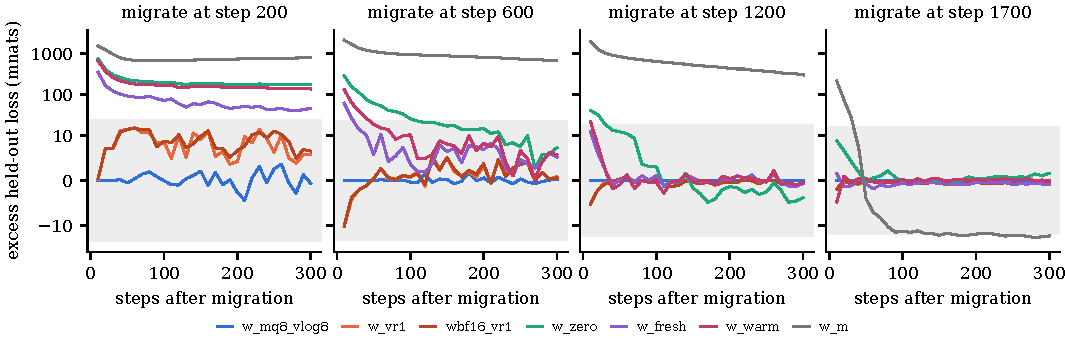
\includegraphics[width=\textwidth]{curves}
\caption{Excess held-out loss after a migration at four points in training (\paramsM{}M parameters, mean over seeds;
the vertical axis is linear within $\pm10$\mnats{} and logarithmic outside). The grey band is $\pm\eps$, the spread
between seeds of the uninterrupted run.}
\label{fig:curves}
\end{figure*}

\subsection{What must cross}
\label{sec:main}

Pending.


\begin{figure*}[t]
\centering
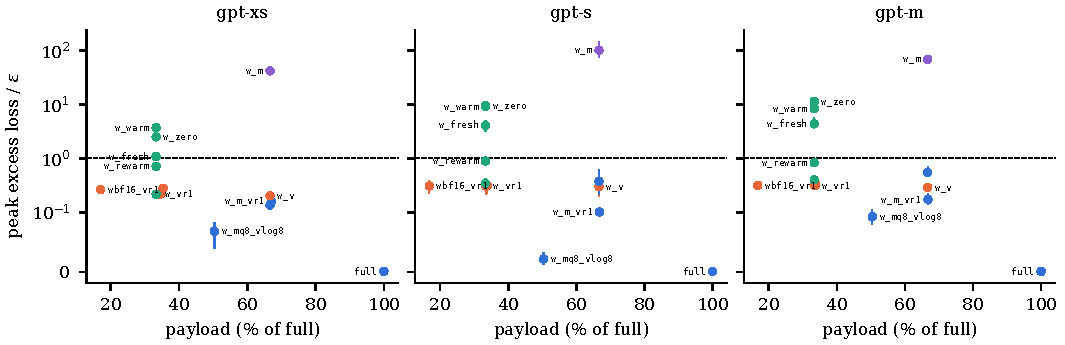
\includegraphics[width=\textwidth]{frontier}
\caption{Bytes against damage at the three model sizes. Each point is a strategy; the horizontal axis is its payload
as a share of the full state, the vertical axis its peak excess loss in units of the seed band, with 95\% intervals.
The dashed line is the noise floor.}
\label{fig:frontier}
\end{figure*}

\begin{table*}[t]
\caption{Peak excess held-out loss in mnats by migration point (\paramsM{}M parameters), with the seed band of each
point in the first row.}
\label{tab:fork}
\centering
\footnotesize
\begin{tabular}{@{}lrrrr@{}}
\toprule
Strategy & Step 200 (10\%) & Step 600 (30\%) & Step 1200 (60\%) & Step 1700 (85\%) \\
\midrule
\gen{tab_fork}
\bottomrule
\end{tabular}
\end{table*}

\subsection{When it matters}
\label{sec:fork}

Pending.


\subsection{First-update diagnostics}
\label{sec:diag}

\begin{table}[t]
\caption{The first update after arrival against the true one (\paramsM{}M, mean over migration points). cos: cosine
with the control's update. Size: norm ratio. $|m|$: norm of the installed first moment over the true one.
$\sqrt{v}$ err: median relative error of the installed $\sqrt{v}$, in percent. The last four columns split cosine and
error into matrices (mat.) and embedding tensors (emb.).}
\label{tab:diag}
\centering
\footnotesize
\setlength{\tabcolsep}{2.6pt}
\begin{tabular}{@{}lrrrrrrrr@{}}
\toprule
 & & & & & \multicolumn{2}{c}{cos} & \multicolumn{2}{c}{$\sqrt{v}$ err} \\
\cmidrule(lr){6-7}\cmidrule(l){8-9}
Strategy & cos & Size & $|m|$ & $\sqrt{v}$ err & mat. & emb. & mat. & emb. \\
\midrule
\gen{tab_diag}
\bottomrule
\end{tabular}
\end{table}

Pending.


\subsection{Sensitivity to the second-moment horizon}
\label{sec:beta}

\begin{table*}[t]
\caption{Peak excess loss over the seed band at three values of $\beta_2$ (\paramsS{}M parameters, migration at 10\% and
60\% of the schedule; \betaSeeds{} seeds for the outer columns). Each value is followed by the number of runs that never
left the band.}
\label{tab:beta}
\centering
\footnotesize
\begin{tabular}{@{}lrcrcrc@{}}
\toprule
 & \multicolumn{2}{c}{$\beta_2 = 0.95$} & \multicolumn{2}{c}{$\beta_2 = 0.99$} & \multicolumn{2}{c}{$\beta_2 = 0.999$} \\
\cmidrule(lr){2-3}\cmidrule(lr){4-5}\cmidrule(l){6-7}
Strategy & Peak/$\eps$ & StR\,$=0$ & Peak/$\eps$ & StR\,$=0$ & Peak/$\eps$ & StR\,$=0$ \\
\midrule
\gen{tab_beta}
\bottomrule
\end{tabular}
\end{table*}

Pending.


\subsection{Drain and restore latency}
\label{sec:latency}

\begin{table*}[t]
\caption{Latency of one migration in milliseconds on the discrete GPU (\paramsM{}M parameters, median of \latReps{}
rounds after warm-up rounds; brackets are the 5th and 95th percentiles). Drain is everything the source does inside the
notice window; restore is everything the destination does before its first step.}
\label{tab:latency}
\centering
\footnotesize
\setlength{\tabcolsep}{4pt}
\begin{tabular}{@{}lrrrrrrrrrrr@{}}
\toprule
 & & \multicolumn{5}{c}{Drain (source)} & \multicolumn{5}{c}{Restore (destination)} \\
\cmidrule(lr){3-7}\cmidrule(l){8-12}
Strategy & MB & encode & to host & serialise & write & total & read & to device & decode & rebuild & total \\
\midrule
\gen{tab_latency}
\bottomrule
\end{tabular}
\end{table*}

Pending.


\subsection{Across device classes}
\label{sec:device}

\begin{table}[t]
\caption{The \arm{full} payload, written on the discrete GPU, resumed on other devices. Gaps are held-out loss
against the same payload resumed on the discrete GPU, in mnats, over 200 steps. \texttt{fp32\_nodrop}: single
precision, no dropout. \texttt{as\_trained}: bfloat16 autocast and dropout, as in the main sweep.}
\label{tab:device}
\centering
\footnotesize
\setlength{\tabcolsep}{2.8pt}
\begin{tabular}{@{}lrllrrrrr@{}}
\toprule
Model & Step & Device & Condition & Arrival & Mean & Max & $\eps$ & Max/$\eps$ \\
\midrule
\gen{tab_device}
\bottomrule
\end{tabular}
\end{table}

Pending.


\subsection{End-to-end preemption}
\label{sec:chaos}

\begin{table*}[t]
\caption{Injected preemptions and crashes during one training run on the discrete GPU. A preemption drains
\arm{w\_vr1} on notice; a crash falls back to the last periodic \arm{w\_mq8\_vlog8} checkpoint. Times in seconds unless
marked.}
\label{tab:chaos}
\centering
\footnotesize
\begin{tabular}{@{}lrlrrrrrrrr@{}}
\toprule
Event & Step & World & Steps redone & Payload (MB) & Drain & Restart & Init & Fetch (ms) & Rebuild (ms) & Downtime \\
\midrule
\gen{tab_chaos_gpu}
\bottomrule
\end{tabular}
\end{table*}

Pending.

